% Created by tikzDevice version 0.12.3.1 on 2022-04-16 20:11:30
% !TEX encoding = UTF-8 Unicode
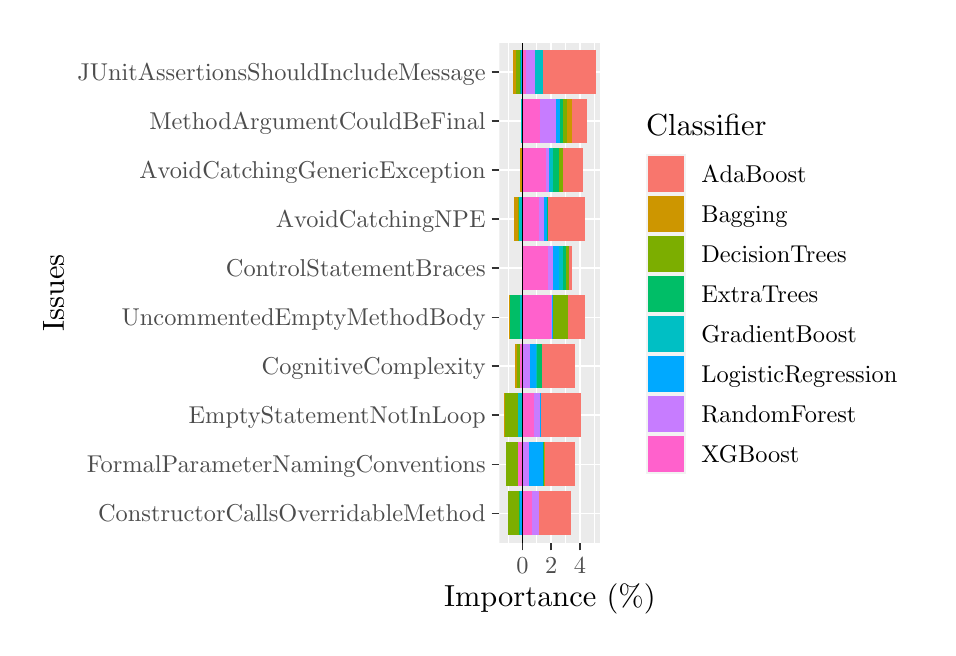
\begin{tikzpicture}[x=1pt,y=1pt]
\definecolor{fillColor}{RGB}{255,255,255}
\path[use as bounding box,fill=fillColor,fill opacity=0.00] (0,0) rectangle (325.21,216.81);
\begin{scope}
\path[clip] (  0.00,  0.00) rectangle (325.21,216.81);
\definecolor{drawColor}{RGB}{255,255,255}
\definecolor{fillColor}{RGB}{255,255,255}

\path[draw=drawColor,line width= 0.6pt,line join=round,line cap=round,fill=fillColor] (  0.00,  0.00) rectangle (325.21,216.81);
\end{scope}
\begin{scope}
\path[clip] (170.43, 30.69) rectangle (206.96,211.31);
\definecolor{fillColor}{gray}{0.92}

\path[fill=fillColor] (170.43, 30.69) rectangle (206.96,211.31);
\definecolor{drawColor}{RGB}{255,255,255}

\path[draw=drawColor,line width= 0.3pt,line join=round] (173.64, 30.69) --
	(173.64,211.31);

\path[draw=drawColor,line width= 0.3pt,line join=round] (184.00, 30.69) --
	(184.00,211.31);

\path[draw=drawColor,line width= 0.3pt,line join=round] (194.37, 30.69) --
	(194.37,211.31);

\path[draw=drawColor,line width= 0.3pt,line join=round] (204.73, 30.69) --
	(204.73,211.31);

\path[draw=drawColor,line width= 0.6pt,line join=round] (170.43, 41.31) --
	(206.96, 41.31);

\path[draw=drawColor,line width= 0.6pt,line join=round] (170.43, 59.02) --
	(206.96, 59.02);

\path[draw=drawColor,line width= 0.6pt,line join=round] (170.43, 76.73) --
	(206.96, 76.73);

\path[draw=drawColor,line width= 0.6pt,line join=round] (170.43, 94.44) --
	(206.96, 94.44);

\path[draw=drawColor,line width= 0.6pt,line join=round] (170.43,112.14) --
	(206.96,112.14);

\path[draw=drawColor,line width= 0.6pt,line join=round] (170.43,129.85) --
	(206.96,129.85);

\path[draw=drawColor,line width= 0.6pt,line join=round] (170.43,147.56) --
	(206.96,147.56);

\path[draw=drawColor,line width= 0.6pt,line join=round] (170.43,165.27) --
	(206.96,165.27);

\path[draw=drawColor,line width= 0.6pt,line join=round] (170.43,182.98) --
	(206.96,182.98);

\path[draw=drawColor,line width= 0.6pt,line join=round] (170.43,200.69) --
	(206.96,200.69);

\path[draw=drawColor,line width= 0.6pt,line join=round] (178.82, 30.69) --
	(178.82,211.31);

\path[draw=drawColor,line width= 0.6pt,line join=round] (189.19, 30.69) --
	(189.19,211.31);

\path[draw=drawColor,line width= 0.6pt,line join=round] (199.55, 30.69) --
	(199.55,211.31);
\definecolor{fillColor}{RGB}{248,118,109}

\path[fill=fillColor] (186.08,192.72) rectangle (205.30,208.65);

\path[fill=fillColor] (196.65,175.01) rectangle (202.04,190.95);

\path[fill=fillColor] (193.33,157.30) rectangle (200.53,173.24);

\path[fill=fillColor] (187.94,139.59) rectangle (201.47,155.53);

\path[fill=fillColor] (195.77,121.88) rectangle (196.65,137.82);

\path[fill=fillColor] (195.40,104.18) rectangle (201.42,120.11);

\path[fill=fillColor] (185.71, 86.47) rectangle (197.68,102.40);

\path[fill=fillColor] (185.66, 68.76) rectangle (200.12, 84.70);

\path[fill=fillColor] (186.85, 51.05) rectangle (197.89, 66.99);

\path[fill=fillColor] (184.73, 33.34) rectangle (196.39, 49.28);
\definecolor{fillColor}{RGB}{205,150,0}

\path[fill=fillColor] (175.25,192.72) rectangle (176.28,208.65);

\path[fill=fillColor] (194.94,175.01) rectangle (196.65,190.95);

\path[fill=fillColor] (178.05,157.30) rectangle (178.82,173.24);

\path[fill=fillColor] (175.66,139.59) rectangle (177.16,155.53);

\path[fill=fillColor] (178.72,121.88) rectangle (178.82,137.82);

\path[fill=fillColor] (173.80,104.18) rectangle (174.31,120.11);

\path[fill=fillColor] (176.18, 86.47) rectangle (176.70,102.40);

\path[fill=fillColor] (172.09, 68.76) rectangle (172.45, 84.70);

\path[fill=fillColor] (186.65, 51.05) rectangle (186.85, 66.99);

\path[fill=fillColor] (173.69, 33.34) rectangle (173.74, 49.28);
\definecolor{fillColor}{RGB}{124,174,0}

\path[fill=fillColor] (176.28,192.72) rectangle (177.84,208.65);

\path[fill=fillColor] (193.33,175.01) rectangle (194.94,190.95);

\path[fill=fillColor] (191.83,157.30) rectangle (193.33,173.24);

\path[fill=fillColor] (177.16,139.59) rectangle (177.68,155.53);

\path[fill=fillColor] (194.68,121.88) rectangle (195.77,137.82);

\path[fill=fillColor] (189.60,104.18) rectangle (195.40,120.11);

\path[fill=fillColor] (176.70, 86.47) rectangle (177.89,102.40);

\path[fill=fillColor] (172.45, 68.76) rectangle (177.01, 84.70);

\path[fill=fillColor] (172.81, 51.05) rectangle (177.01, 66.99);

\path[fill=fillColor] (173.74, 33.34) rectangle (177.53, 49.28);
\definecolor{fillColor}{RGB}{0,190,103}

\path[fill=fillColor] (177.84,192.72) rectangle (178.41,208.65);

\path[fill=fillColor] (192.45,175.01) rectangle (193.33,190.95);

\path[fill=fillColor] (189.70,157.30) rectangle (191.83,173.24);

\path[fill=fillColor] (187.53,139.59) rectangle (187.94,155.53);

\path[fill=fillColor] (193.54,121.88) rectangle (194.68,137.82);

\path[fill=fillColor] (174.31,104.18) rectangle (177.84,120.11);

\path[fill=fillColor] (184.16, 86.47) rectangle (185.71,102.40);

\path[fill=fillColor] (177.01, 68.76) rectangle (177.06, 84.70);

\path[fill=fillColor] (186.13, 51.05) rectangle (186.65, 66.99);

\path[fill=fillColor] (177.53, 33.34) rectangle (177.84, 49.28);
\definecolor{fillColor}{RGB}{0,191,196}

\path[fill=fillColor] (183.28,192.72) rectangle (186.08,208.65);

\path[fill=fillColor] (178.10,175.01) rectangle (178.82,190.95);

\path[fill=fillColor] (188.41,157.30) rectangle (189.70,173.24);

\path[fill=fillColor] (177.68,139.59) rectangle (178.82,155.53);

\path[fill=fillColor] (192.14,121.88) rectangle (193.54,137.82);

\path[fill=fillColor] (177.84,104.18) rectangle (178.82,120.11);

\path[fill=fillColor] (183.69, 86.47) rectangle (184.16,102.40);

\path[fill=fillColor] (177.06, 68.76) rectangle (178.82, 84.70);

\path[fill=fillColor] (177.01, 51.05) rectangle (177.16, 66.99);

\path[fill=fillColor] (177.84, 33.34) rectangle (177.94, 49.28);
\definecolor{fillColor}{RGB}{0,169,255}

\path[fill=fillColor] (178.41,192.72) rectangle (178.82,208.65);

\path[fill=fillColor] (190.74,175.01) rectangle (192.45,190.95);

\path[fill=fillColor] (188.36,157.30) rectangle (188.41,173.24);

\path[fill=fillColor] (186.70,139.59) rectangle (187.53,155.53);

\path[fill=fillColor] (189.91,121.88) rectangle (192.14,137.82);

\path[fill=fillColor] (189.39,104.18) rectangle (189.60,120.11);

\path[fill=fillColor] (181.62, 86.47) rectangle (183.69,102.40);

\path[fill=fillColor] (185.04, 68.76) rectangle (185.66, 84.70);

\path[fill=fillColor] (181.26, 51.05) rectangle (186.13, 66.99);

\path[fill=fillColor] (177.94, 33.34) rectangle (178.82, 49.28);
\definecolor{fillColor}{RGB}{199,124,255}

\path[fill=fillColor] (180.17,192.72) rectangle (183.28,208.65);

\path[fill=fillColor] (185.25,175.01) rectangle (190.74,190.95);

\path[fill=fillColor] (187.32,157.30) rectangle (188.36,173.24);

\path[fill=fillColor] (184.83,139.59) rectangle (186.70,155.53);

\path[fill=fillColor] (187.99,121.88) rectangle (189.91,137.82);

\path[fill=fillColor] (188.93,104.18) rectangle (189.39,120.11);

\path[fill=fillColor] (178.82, 86.47) rectangle (181.62,102.40);

\path[fill=fillColor] (182.86, 68.76) rectangle (185.04, 84.70);

\path[fill=fillColor] (178.82, 51.05) rectangle (181.26, 66.99);

\path[fill=fillColor] (182.19, 33.34) rectangle (184.73, 49.28);
\definecolor{fillColor}{RGB}{255,97,204}

\path[fill=fillColor] (178.82,192.72) rectangle (180.17,208.65);

\path[fill=fillColor] (178.82,175.01) rectangle (185.25,190.95);

\path[fill=fillColor] (178.82,157.30) rectangle (187.32,173.24);

\path[fill=fillColor] (178.82,139.59) rectangle (184.83,155.53);

\path[fill=fillColor] (178.82,121.88) rectangle (187.99,137.82);

\path[fill=fillColor] (178.82,104.18) rectangle (188.93,120.11);

\path[fill=fillColor] (177.89, 86.47) rectangle (178.82,102.40);

\path[fill=fillColor] (178.82, 68.76) rectangle (182.86, 84.70);

\path[fill=fillColor] (177.16, 51.05) rectangle (178.82, 66.99);

\path[fill=fillColor] (178.82, 33.34) rectangle (182.19, 49.28);
\definecolor{drawColor}{RGB}{0,0,0}

\path[draw=drawColor,line width= 0.6pt,line join=round] (178.82, 30.69) -- (178.82,211.31);
\end{scope}
\begin{scope}
\path[clip] (  0.00,  0.00) rectangle (325.21,216.81);
\definecolor{drawColor}{gray}{0.30}

\node[text=drawColor,anchor=base east,inner sep=0pt, outer sep=0pt, scale=  0.88] at (165.48, 38.28) {ConstructorCallsOverridableMethod};

\node[text=drawColor,anchor=base east,inner sep=0pt, outer sep=0pt, scale=  0.88] at (165.48, 55.99) {FormalParameterNamingConventions};

\node[text=drawColor,anchor=base east,inner sep=0pt, outer sep=0pt, scale=  0.88] at (165.48, 73.70) {EmptyStatementNotInLoop};

\node[text=drawColor,anchor=base east,inner sep=0pt, outer sep=0pt, scale=  0.88] at (165.48, 91.41) {CognitiveComplexity};

\node[text=drawColor,anchor=base east,inner sep=0pt, outer sep=0pt, scale=  0.88] at (165.48,109.11) {UncommentedEmptyMethodBody};

\node[text=drawColor,anchor=base east,inner sep=0pt, outer sep=0pt, scale=  0.88] at (165.48,126.82) {ControlStatementBraces};

\node[text=drawColor,anchor=base east,inner sep=0pt, outer sep=0pt, scale=  0.88] at (165.48,144.53) {AvoidCatchingNPE};

\node[text=drawColor,anchor=base east,inner sep=0pt, outer sep=0pt, scale=  0.88] at (165.48,162.24) {AvoidCatchingGenericException};

\node[text=drawColor,anchor=base east,inner sep=0pt, outer sep=0pt, scale=  0.88] at (165.48,179.95) {MethodArgumentCouldBeFinal};

\node[text=drawColor,anchor=base east,inner sep=0pt, outer sep=0pt, scale=  0.88] at (165.48,197.65) {JUnitAssertionsShouldIncludeMessage};
\end{scope}
\begin{scope}
\path[clip] (  0.00,  0.00) rectangle (325.21,216.81);
\definecolor{drawColor}{gray}{0.20}

\path[draw=drawColor,line width= 0.6pt,line join=round] (167.68, 41.31) --
	(170.43, 41.31);

\path[draw=drawColor,line width= 0.6pt,line join=round] (167.68, 59.02) --
	(170.43, 59.02);

\path[draw=drawColor,line width= 0.6pt,line join=round] (167.68, 76.73) --
	(170.43, 76.73);

\path[draw=drawColor,line width= 0.6pt,line join=round] (167.68, 94.44) --
	(170.43, 94.44);

\path[draw=drawColor,line width= 0.6pt,line join=round] (167.68,112.14) --
	(170.43,112.14);

\path[draw=drawColor,line width= 0.6pt,line join=round] (167.68,129.85) --
	(170.43,129.85);

\path[draw=drawColor,line width= 0.6pt,line join=round] (167.68,147.56) --
	(170.43,147.56);

\path[draw=drawColor,line width= 0.6pt,line join=round] (167.68,165.27) --
	(170.43,165.27);

\path[draw=drawColor,line width= 0.6pt,line join=round] (167.68,182.98) --
	(170.43,182.98);

\path[draw=drawColor,line width= 0.6pt,line join=round] (167.68,200.69) --
	(170.43,200.69);
\end{scope}
\begin{scope}
\path[clip] (  0.00,  0.00) rectangle (325.21,216.81);
\definecolor{drawColor}{gray}{0.20}

\path[draw=drawColor,line width= 0.6pt,line join=round] (178.82, 27.94) --
	(178.82, 30.69);

\path[draw=drawColor,line width= 0.6pt,line join=round] (189.19, 27.94) --
	(189.19, 30.69);

\path[draw=drawColor,line width= 0.6pt,line join=round] (199.55, 27.94) --
	(199.55, 30.69);
\end{scope}
\begin{scope}
\path[clip] (  0.00,  0.00) rectangle (325.21,216.81);
\definecolor{drawColor}{gray}{0.30}

\node[text=drawColor,anchor=base,inner sep=0pt, outer sep=0pt, scale=  0.88] at (178.82, 19.68) {0};

\node[text=drawColor,anchor=base,inner sep=0pt, outer sep=0pt, scale=  0.88] at (189.19, 19.68) {2};

\node[text=drawColor,anchor=base,inner sep=0pt, outer sep=0pt, scale=  0.88] at (199.55, 19.68) {4};
\end{scope}
\begin{scope}
\path[clip] (  0.00,  0.00) rectangle (325.21,216.81);
\definecolor{drawColor}{RGB}{0,0,0}

\node[text=drawColor,anchor=base,inner sep=0pt, outer sep=0pt, scale=  1.10] at (188.69,  7.64) {Importance (\%)};
\end{scope}
\begin{scope}
\path[clip] (  0.00,  0.00) rectangle (325.21,216.81);
\definecolor{drawColor}{RGB}{0,0,0}

\node[text=drawColor,rotate= 90.00,anchor=base,inner sep=0pt, outer sep=0pt, scale=  1.10] at ( 13.08,121.00) {Issues};
\end{scope}
\begin{scope}
\path[clip] (  0.00,  0.00) rectangle (325.21,216.81);
\definecolor{fillColor}{RGB}{255,255,255}

\path[fill=fillColor] (217.96, 50.07) rectangle (319.71,191.92);
\end{scope}
\begin{scope}
\path[clip] (  0.00,  0.00) rectangle (325.21,216.81);
\definecolor{drawColor}{RGB}{0,0,0}

\node[text=drawColor,anchor=base west,inner sep=0pt, outer sep=0pt, scale=  1.10] at (223.46,177.78) {Classifier};
\end{scope}
\begin{scope}
\path[clip] (  0.00,  0.00) rectangle (325.21,216.81);
\definecolor{fillColor}{gray}{0.95}

\path[fill=fillColor] (223.46,156.75) rectangle (237.92,171.21);
\end{scope}
\begin{scope}
\path[clip] (  0.00,  0.00) rectangle (325.21,216.81);
\definecolor{fillColor}{RGB}{248,118,109}

\path[fill=fillColor] (224.17,157.46) rectangle (237.21,170.50);
\end{scope}
\begin{scope}
\path[clip] (  0.00,  0.00) rectangle (325.21,216.81);
\definecolor{fillColor}{gray}{0.95}

\path[fill=fillColor] (223.46,142.30) rectangle (237.92,156.75);
\end{scope}
\begin{scope}
\path[clip] (  0.00,  0.00) rectangle (325.21,216.81);
\definecolor{fillColor}{RGB}{205,150,0}

\path[fill=fillColor] (224.17,143.01) rectangle (237.21,156.04);
\end{scope}
\begin{scope}
\path[clip] (  0.00,  0.00) rectangle (325.21,216.81);
\definecolor{fillColor}{gray}{0.95}

\path[fill=fillColor] (223.46,127.84) rectangle (237.92,142.30);
\end{scope}
\begin{scope}
\path[clip] (  0.00,  0.00) rectangle (325.21,216.81);
\definecolor{fillColor}{RGB}{124,174,0}

\path[fill=fillColor] (224.17,128.56) rectangle (237.21,141.59);
\end{scope}
\begin{scope}
\path[clip] (  0.00,  0.00) rectangle (325.21,216.81);
\definecolor{fillColor}{gray}{0.95}

\path[fill=fillColor] (223.46,113.39) rectangle (237.92,127.84);
\end{scope}
\begin{scope}
\path[clip] (  0.00,  0.00) rectangle (325.21,216.81);
\definecolor{fillColor}{RGB}{0,190,103}

\path[fill=fillColor] (224.17,114.10) rectangle (237.21,127.13);
\end{scope}
\begin{scope}
\path[clip] (  0.00,  0.00) rectangle (325.21,216.81);
\definecolor{fillColor}{gray}{0.95}

\path[fill=fillColor] (223.46, 98.94) rectangle (237.92,113.39);
\end{scope}
\begin{scope}
\path[clip] (  0.00,  0.00) rectangle (325.21,216.81);
\definecolor{fillColor}{RGB}{0,191,196}

\path[fill=fillColor] (224.17, 99.65) rectangle (237.21,112.68);
\end{scope}
\begin{scope}
\path[clip] (  0.00,  0.00) rectangle (325.21,216.81);
\definecolor{fillColor}{gray}{0.95}

\path[fill=fillColor] (223.46, 84.48) rectangle (237.92, 98.94);
\end{scope}
\begin{scope}
\path[clip] (  0.00,  0.00) rectangle (325.21,216.81);
\definecolor{fillColor}{RGB}{0,169,255}

\path[fill=fillColor] (224.17, 85.19) rectangle (237.21, 98.23);
\end{scope}
\begin{scope}
\path[clip] (  0.00,  0.00) rectangle (325.21,216.81);
\definecolor{fillColor}{gray}{0.95}

\path[fill=fillColor] (223.46, 70.03) rectangle (237.92, 84.48);
\end{scope}
\begin{scope}
\path[clip] (  0.00,  0.00) rectangle (325.21,216.81);
\definecolor{fillColor}{RGB}{199,124,255}

\path[fill=fillColor] (224.17, 70.74) rectangle (237.21, 83.77);
\end{scope}
\begin{scope}
\path[clip] (  0.00,  0.00) rectangle (325.21,216.81);
\definecolor{fillColor}{gray}{0.95}

\path[fill=fillColor] (223.46, 55.57) rectangle (237.92, 70.03);
\end{scope}
\begin{scope}
\path[clip] (  0.00,  0.00) rectangle (325.21,216.81);
\definecolor{fillColor}{RGB}{255,97,204}

\path[fill=fillColor] (224.17, 56.29) rectangle (237.21, 69.32);
\end{scope}
\begin{scope}
\path[clip] (  0.00,  0.00) rectangle (325.21,216.81);
\definecolor{drawColor}{RGB}{0,0,0}

\node[text=drawColor,anchor=base west,inner sep=0pt, outer sep=0pt, scale=  0.88] at (243.42,160.95) {AdaBoost};
\end{scope}
\begin{scope}
\path[clip] (  0.00,  0.00) rectangle (325.21,216.81);
\definecolor{drawColor}{RGB}{0,0,0}

\node[text=drawColor,anchor=base west,inner sep=0pt, outer sep=0pt, scale=  0.88] at (243.42,146.50) {Bagging};
\end{scope}
\begin{scope}
\path[clip] (  0.00,  0.00) rectangle (325.21,216.81);
\definecolor{drawColor}{RGB}{0,0,0}

\node[text=drawColor,anchor=base west,inner sep=0pt, outer sep=0pt, scale=  0.88] at (243.42,132.04) {DecisionTrees};
\end{scope}
\begin{scope}
\path[clip] (  0.00,  0.00) rectangle (325.21,216.81);
\definecolor{drawColor}{RGB}{0,0,0}

\node[text=drawColor,anchor=base west,inner sep=0pt, outer sep=0pt, scale=  0.88] at (243.42,117.59) {ExtraTrees};
\end{scope}
\begin{scope}
\path[clip] (  0.00,  0.00) rectangle (325.21,216.81);
\definecolor{drawColor}{RGB}{0,0,0}

\node[text=drawColor,anchor=base west,inner sep=0pt, outer sep=0pt, scale=  0.88] at (243.42,103.13) {GradientBoost};
\end{scope}
\begin{scope}
\path[clip] (  0.00,  0.00) rectangle (325.21,216.81);
\definecolor{drawColor}{RGB}{0,0,0}

\node[text=drawColor,anchor=base west,inner sep=0pt, outer sep=0pt, scale=  0.88] at (243.42, 88.68) {LogisticRegression};
\end{scope}
\begin{scope}
\path[clip] (  0.00,  0.00) rectangle (325.21,216.81);
\definecolor{drawColor}{RGB}{0,0,0}

\node[text=drawColor,anchor=base west,inner sep=0pt, outer sep=0pt, scale=  0.88] at (243.42, 74.23) {RandomForest};
\end{scope}
\begin{scope}
\path[clip] (  0.00,  0.00) rectangle (325.21,216.81);
\definecolor{drawColor}{RGB}{0,0,0}

\node[text=drawColor,anchor=base west,inner sep=0pt, outer sep=0pt, scale=  0.88] at (243.42, 59.77) {XGBoost};
\end{scope}
\end{tikzpicture}
